\documentclass[12pt]{article} 
\usepackage[utf8]{inputenc}
\usepackage[T2A]{fontenc}
\usepackage{amsthm}
\usepackage{amssymb}
\usepackage{blindtext}
\usepackage{amsmath}
\usepackage{tikz} 
\usepackage{listings}
\usepackage{xcolor}
\usepackage{float}
\usepackage{graphicx}
\usepackage{hyperref}
\hypersetup{
    colorlinks=true,
    linkcolor=blue,
    filecolor=blue,      
    urlcolor=blue,
    pdftitle={Overleaf Example},
    pdfpagemode=FullScreen,
    }
\graphicspath{ {./images} }

\title{Bioinformatics HW2}
\author{Ershov Ivan}
\date{November 2021}

\begin{document}

\maketitle
Выбранный ген - ribosomal protein L6

\paragraph{Задание 1.}
Найдем аминокислотные последовательности генов для различных видов и составим fasta-файл с последовательностями. Поставим в начало названия гена строку с названием организма, чтобы организм в будущем отображался на листьях дерева.\\
Вот ссылки на последовательности, которые я скачал:
\begin{enumerate}
    \itemsep0em
    \item \href{https://www.ncbi.nlm.nih.gov/protein/CAA49188.1?report=fasta}{Человек - human, вид Homo sapiens} 
    \item \href{https://www.ncbi.nlm.nih.gov/protein/NP_001180484.1?report=fasta}{Обезьяна - primates, вид Macaca mulatta} 
    \item \href{https://www.ncbi.nlm.nih.gov/protein/NP_035420.2?report=fasta}{Грузуны(мышь) - mouse, вид Mus musculus} 
    \item \href{https://www.ncbi.nlm.nih.gov/protein/CAA60588.1?report=fasta}{Грузуны(крыса) - rat, вид Rattus norvegicus} 
    \item \href{https://www.ncbi.nlm.nih.gov/protein/AAI33431.1?report=fasta}{Копытное -   bovine, вид Bos taurus} 
    \item \href{https://www.ncbi.nlm.nih.gov/protein/XP_027720672.1?report=fasta}{Cумчатое - marsupials, вид Vombatus ursinus} 
    \item \href{https://www.ncbi.nlm.nih.gov/protein/XP_007433584.1?report=fasta}{Пресмыкающиеся(змея) – snakes, вид Python bivittatus} 
    \item \href{https://www.ncbi.nlm.nih.gov/protein/XP_020657572.1?report=fasta}{Пресмыкающиеся(ящерица) – lizards, вид Pogona vitticeps} 
    \item \href{https://www.ncbi.nlm.nih.gov/protein/EMP37138.1?report=fasta}{Пресмыкающиеся(черепаха) – turtles, вид Chelonia mydas} 
    \item \href{https://www.ncbi.nlm.nih.gov/protein/LAC33108.1?report=fasta}{Птица - bird, вид Gallirallus okinawae} 
    \item \href{https://www.ncbi.nlm.nih.gov/protein/NP_001158741.1?report=fasta}{Рыба - fish, вид Salmo salar} 
    \item \href{https://www.ncbi.nlm.nih.gov/protein/AAW50981.1?report=fasta}{Растение - plant, вид Triticum aestivum} 
    \item \href{https://www.ncbi.nlm.nih.gov/protein/CAA49236.1?report=fasta}{Пекарские дрожжи  - fungi, вид Saccharomyces cerevisiae} 
    \item \href{https://www.ncbi.nlm.nih.gov/protein/ADB58394.1?report=fasta}{Архея - archaea, вид Archaeoglobus profundus DSM 5631} 
    \item \href{https://www.ncbi.nlm.nih.gov/protein/AEW03871.1?report=fasta}{Бактерия –bacteria, вид Sulfobacillus acidophilus DSM 10332} 
\end{enumerate}
\newpage
\paragraph{Задание 2.}
С помощью приложения Mega произведем множественное выравнивание последовательностей алгоритмами ClustalW и Muscle \\
(представлю здесь скриншоты полученных выравниваний. К письму тоже приложу итоговые выравнивания файлами)\\
\subparagraph{Muscle alignment\\}
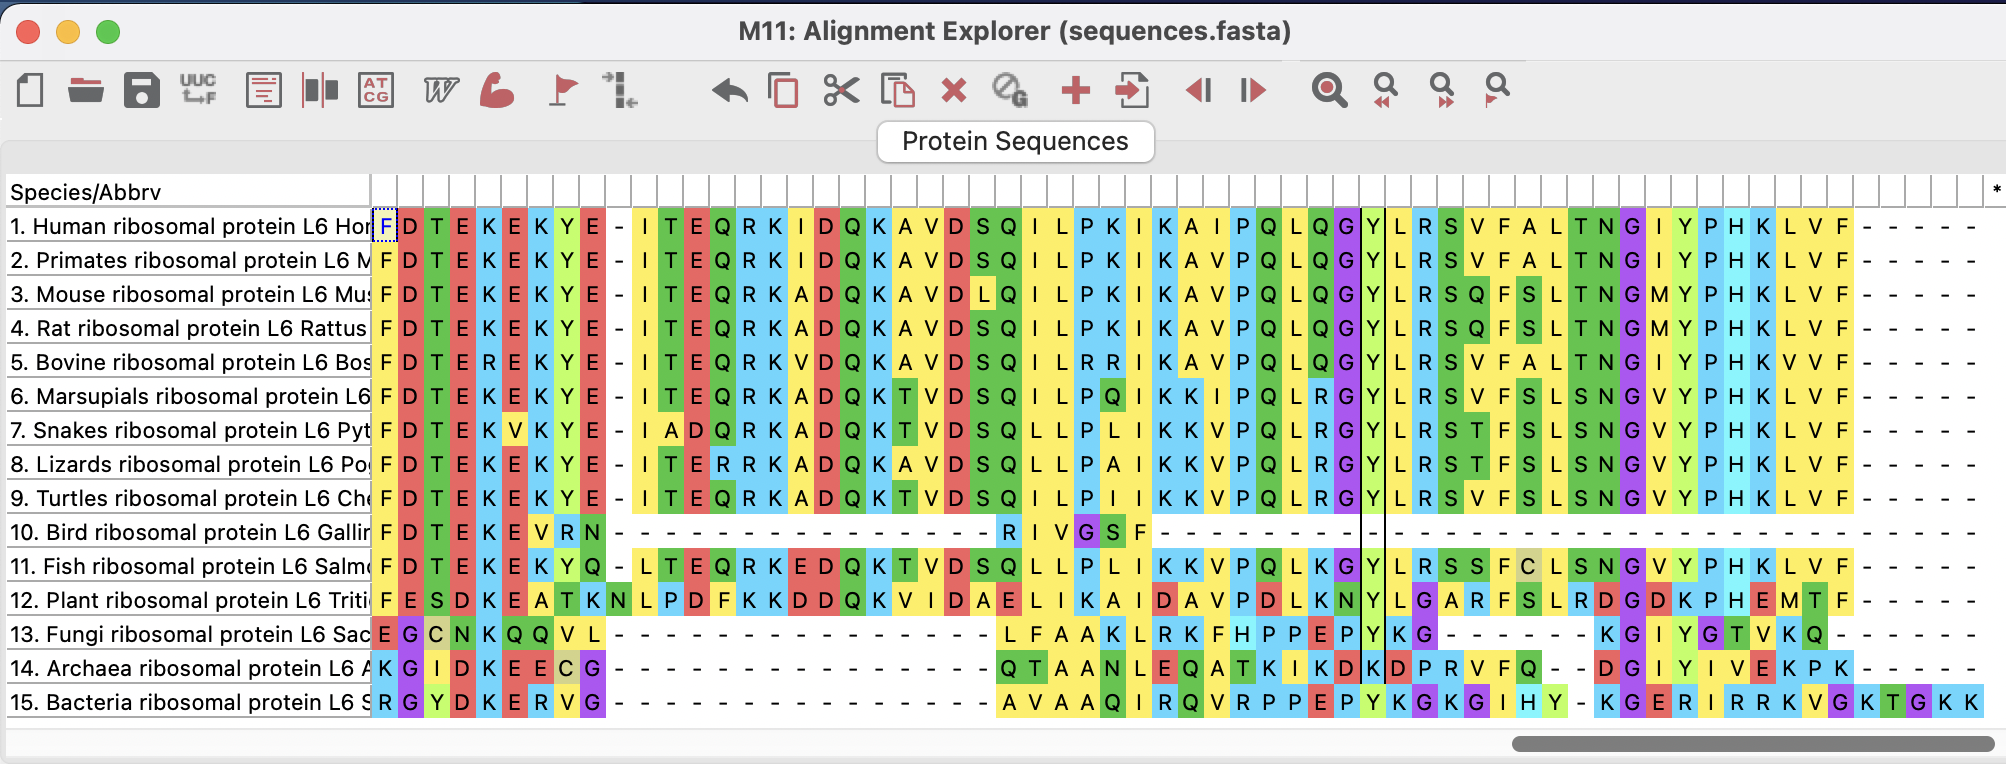
\includegraphics[width=\textwidth]{images/image1.png}\\

\subparagraph{ClustalW alignment\\}
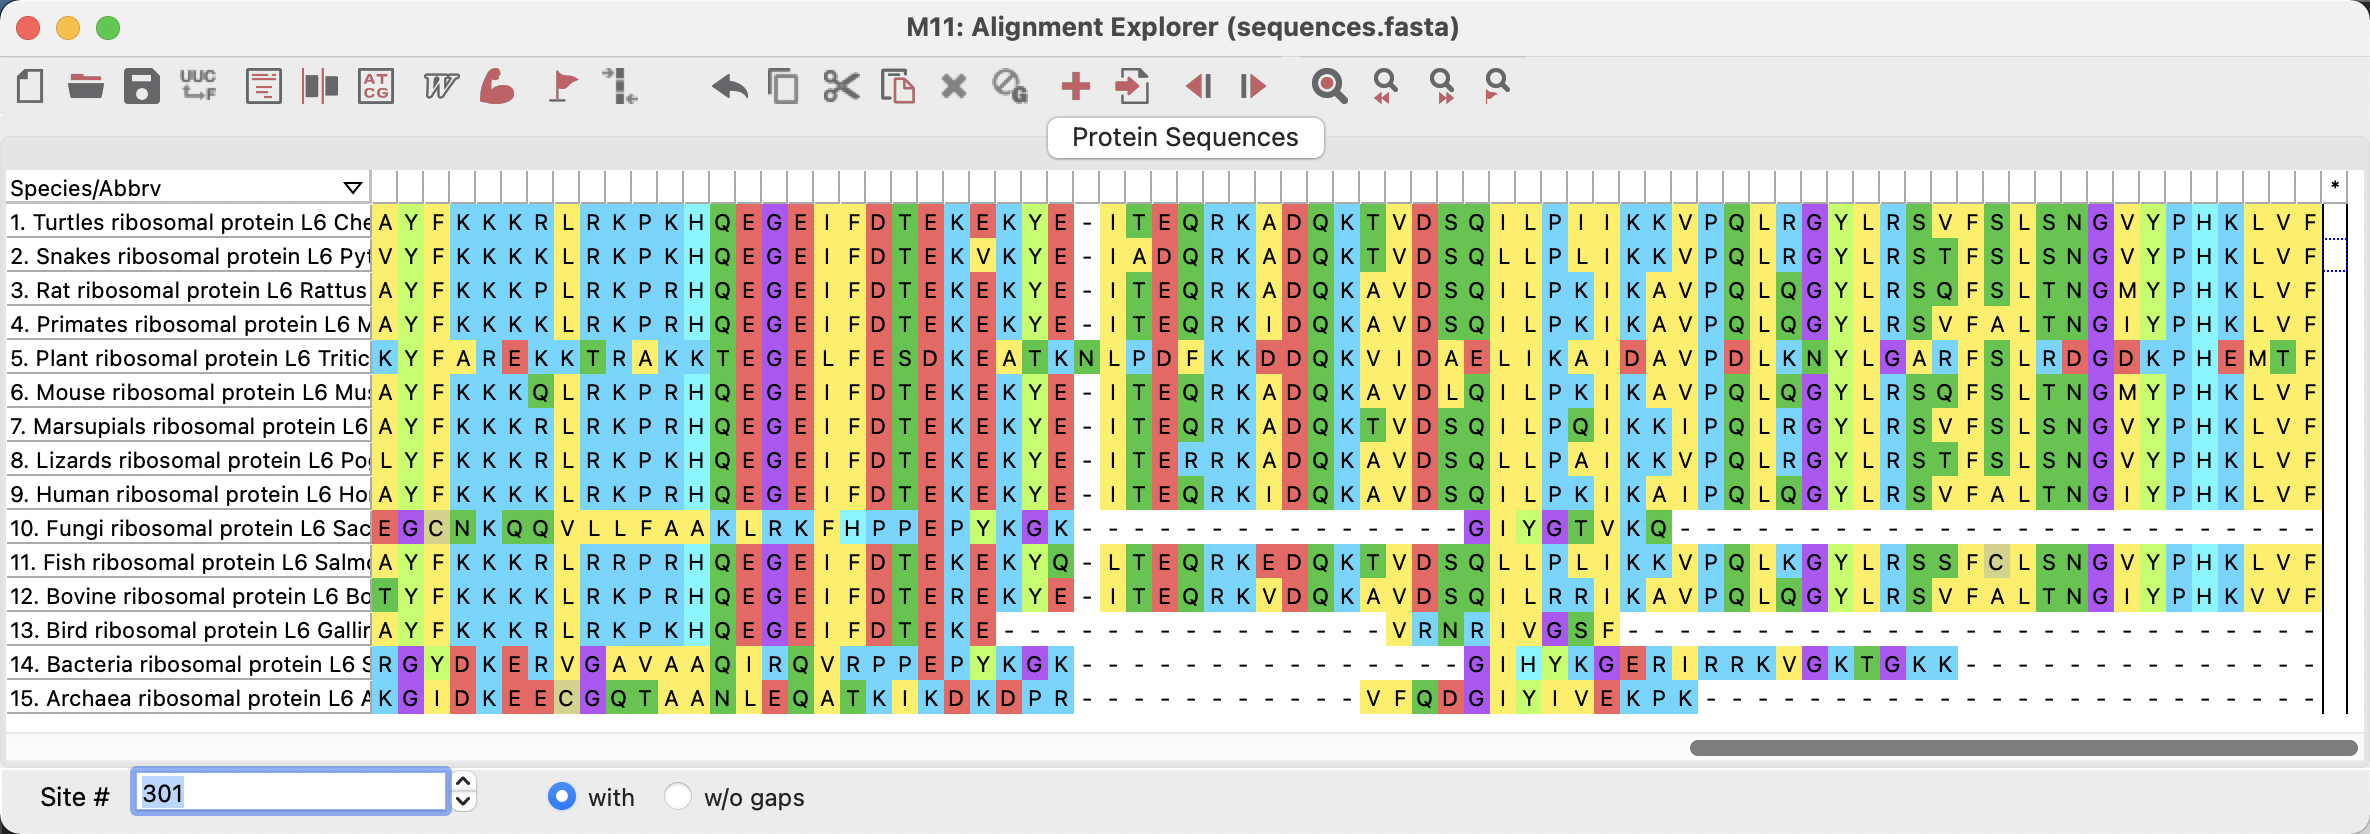
\includegraphics[width=\textwidth]{images/image2.png}\\

Полученные выравнивания отличаются по крайней мере расположением пропусков (это явно видно на скриншотах)

\newpage
\paragraph{Задание 3.}

\subparagraph{Построим деревья для Muscle alignment}
\begin{itemize}
    \itemsep0em
    \item методом расстояний (UPGMA) Bootstrap 100\\
    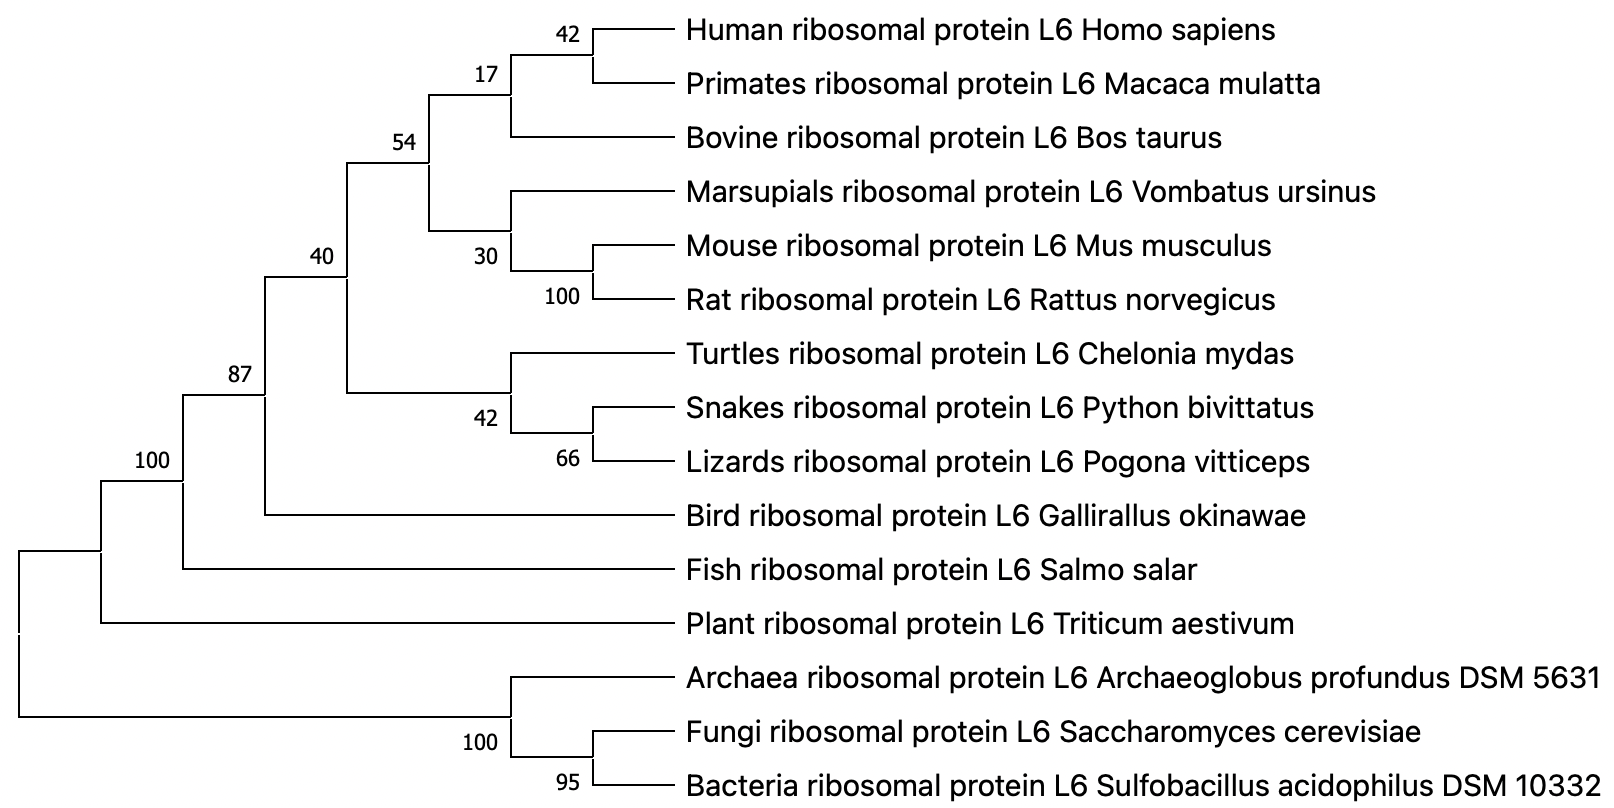
\includegraphics[width=\textwidth]{images/image3.png}\\
    \item методом расстояний (NJ) Bootstrap 100\\
    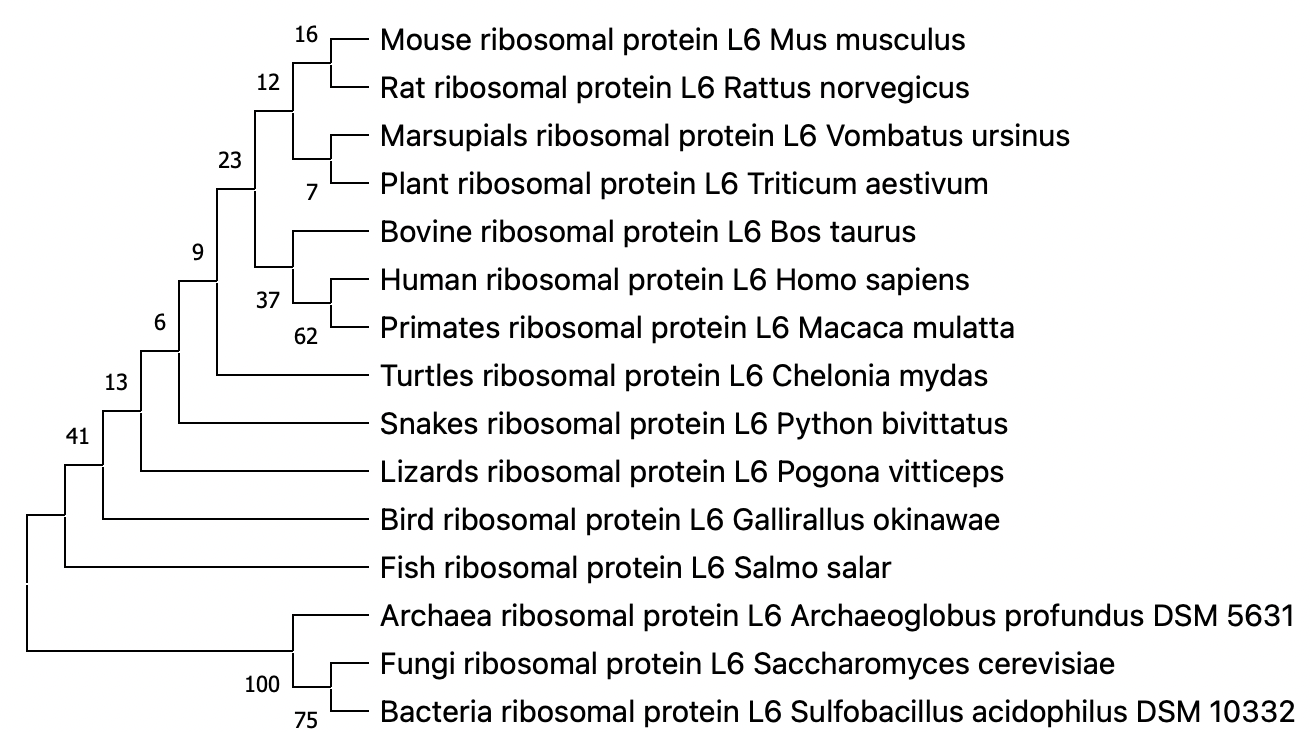
\includegraphics[width=\textwidth]{images/image4.png}\\
    \newpage
    \item методом максимального правдоподобия Bootstrap 100\\
    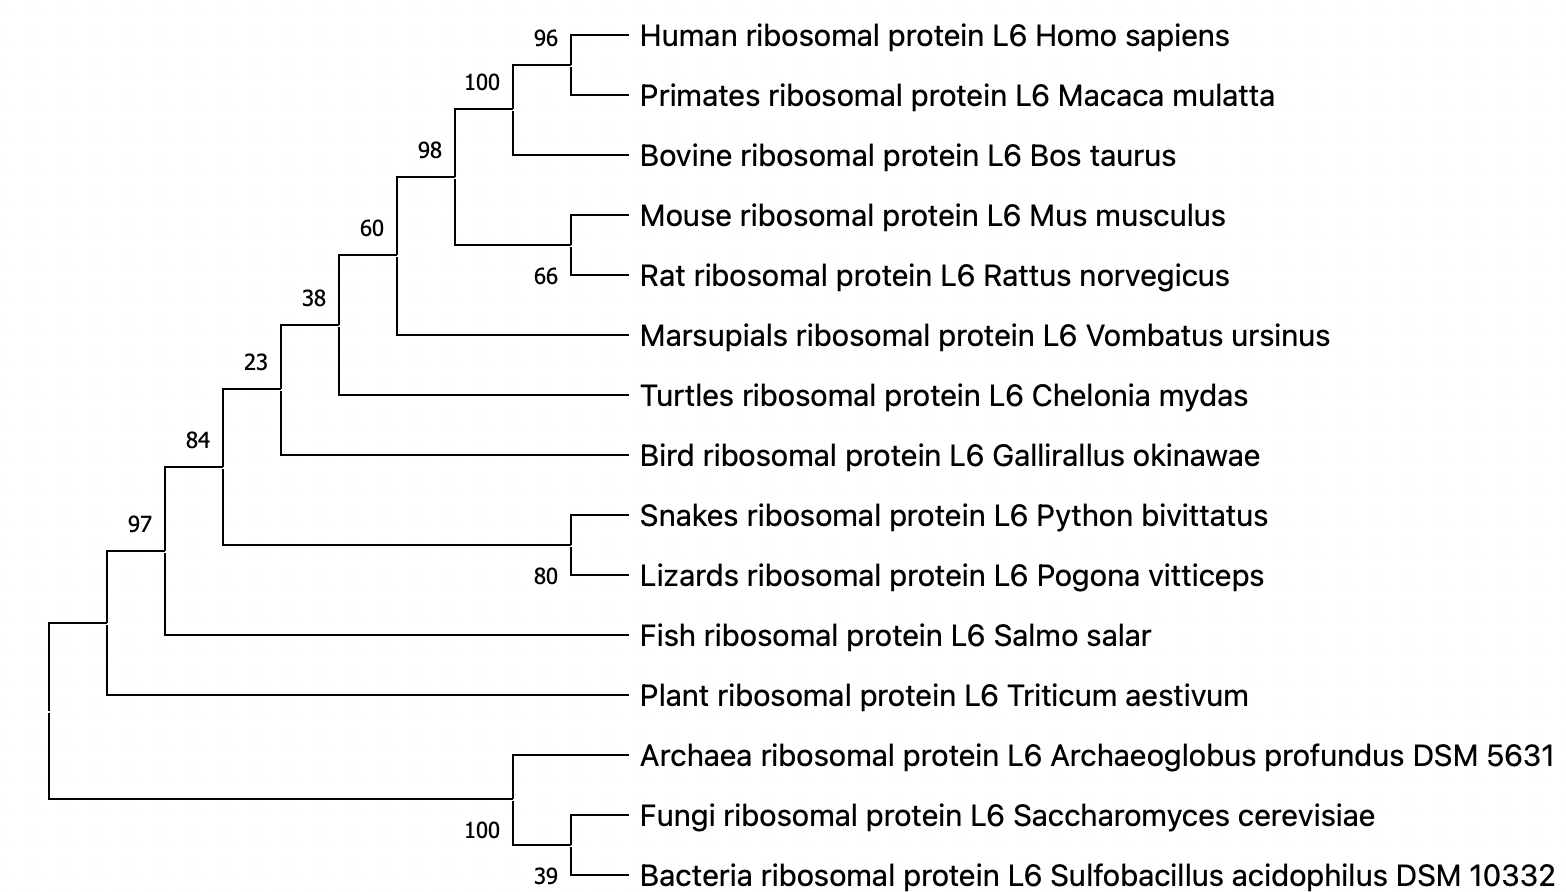
\includegraphics[width=\textwidth]{images/image5.png}\\
\end{itemize}

\subparagraph{Построим деревья для ClustalW alignment}
\begin{itemize}
    \itemsep0em
    \item методом расстояний (UPGMA) Bootstrap 100\\
    
\includegraphics[width=\textwidth]{images/image6.png}\\
    \newpage
    \item методом расстояний (NJ) Bootstrap 100\\
    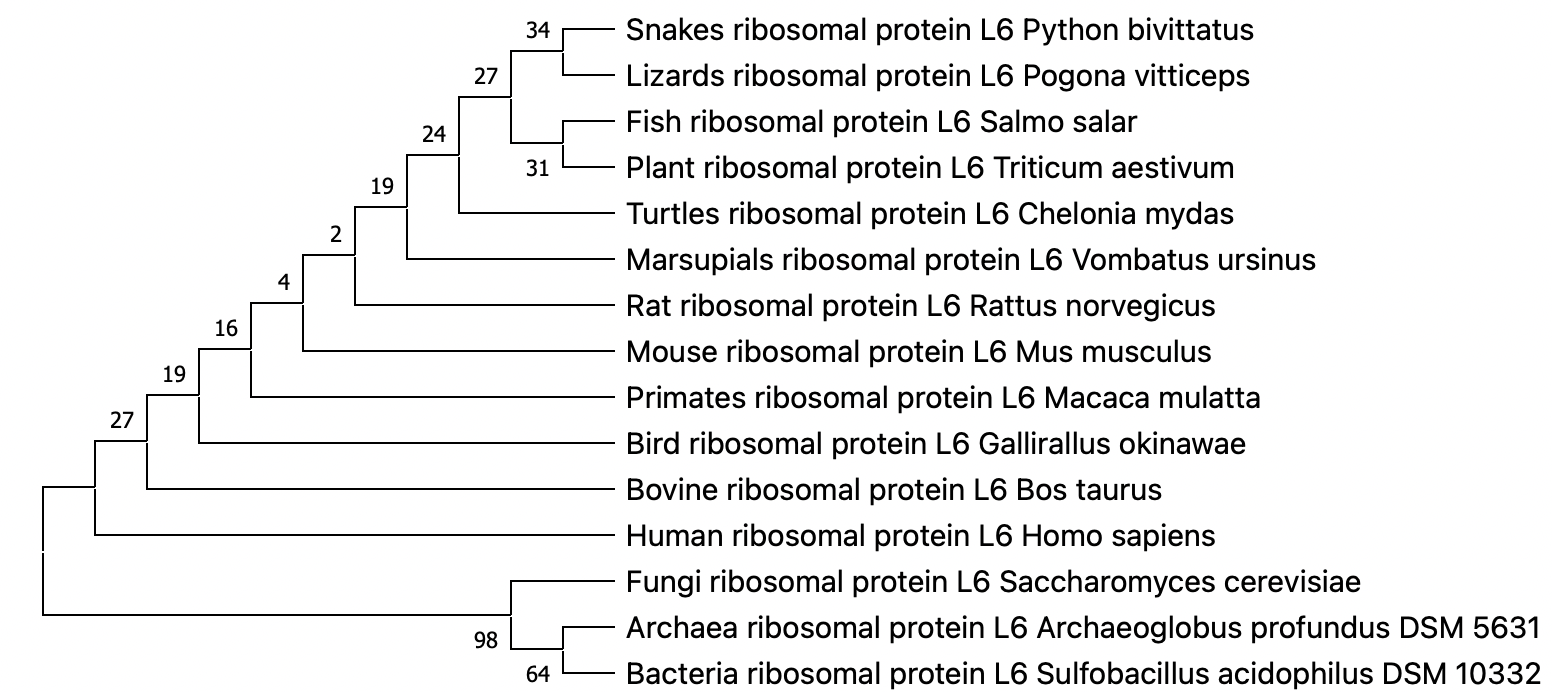
\includegraphics[width=\textwidth]{images/image7.png}\\
    \item методом максимального правдоподобия Bootstrap 100\\
    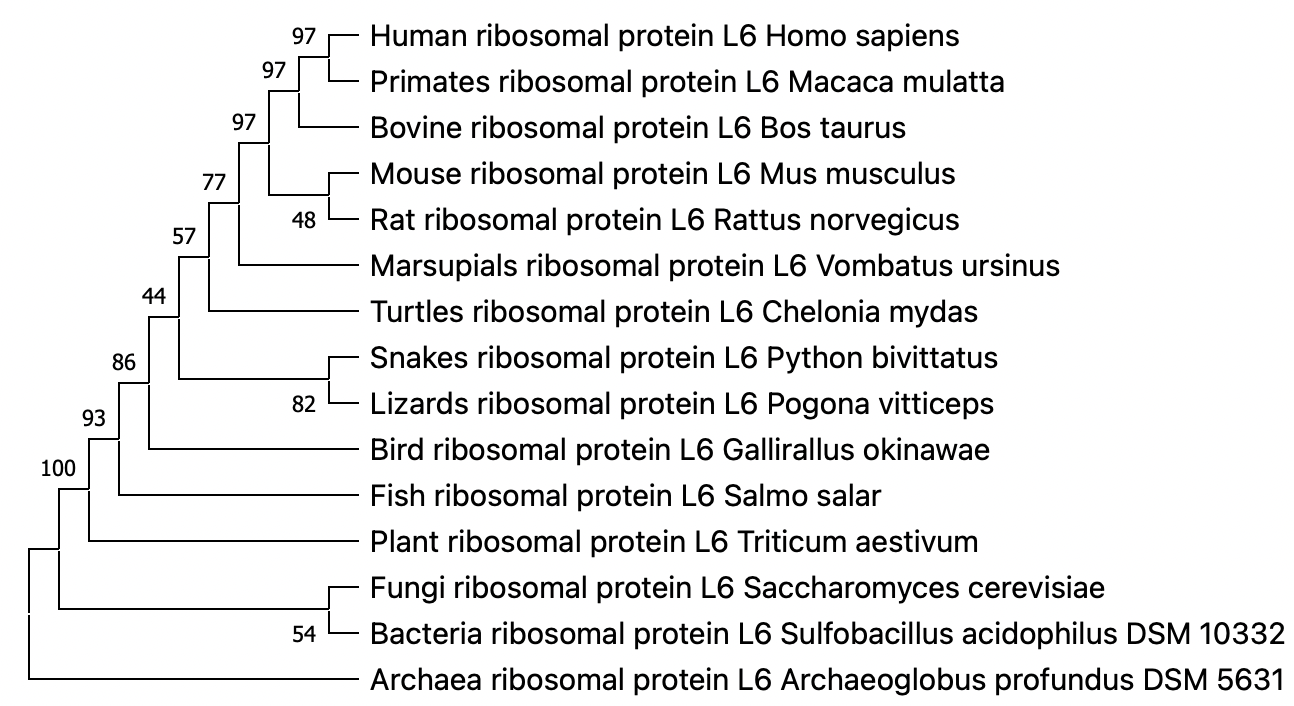
\includegraphics[width=\textwidth]{images/image8.png}\\
\end{itemize}
\newpage
\paragraph{Вывод:}
\subparagraph{Какой алгоритм выравнивания лучше сработал -  ClustalW или Muscle?\\}
Сложно сравнивать два этих алгоритма, но, мне кажется, метод Muscle отработал лучше. Дерево, постороенное методом расстояний (NJ) с ClustalW, обладает маленьким количеством различных развлетлений, разные виды по больше части соединеные последовательно, а некоторые виды, которые, казалось бы должны быть вместе, такие как ящерица, змея и черепаха, расположились даже не близко, В это же время в Muscle тот же метод объединил по крайней мере мышь и крысу, а уже упомянутые змеи, ящерицы и черепахи расположены близко.

\subparagraph{Одинаковая ли получилась топология деревьев при построении разными методами?\\}
В целом, можно заметить, что у деревьев построенных одним методом, но для последовательностей выравненных по-разному, имеют сходства в узлах и ветвях. Некоторые деревья (например построенные методом расстояний UPGMA) очень похожи (хотя опять же, не идентичны), а некторые скорее непохожи (как описанные в предыдещем пункте деревья, построенные при помощи NJ) и имеют мало сходств.

\subparagraph{Одинаковые ли получились бутстрэп-значения?\\}
Ответ в большинстве случаев нет, для этого достаточно взглянуть на построенные деревья и удостовериться в этом. Однако почти все бутстрэп-значения деревьев, построенные одним методом, но разными выравниваниями, различаеются в $\pm$ 20.

\subparagraph{Совпадают ли деревья, построенные по одному гену с принятыми деревьями видов?\\}
Eсть принятая таксономия, как произошли виды. Она составлена на основе, как и обычной биологии, так и молекулярной биологии. На сайте NCBI можно построить дерево таксономии по выбранным видам организмов. Я так и сделал и объединил выбранные мной виды в дерево (дерево на следующей странице)
\newpage
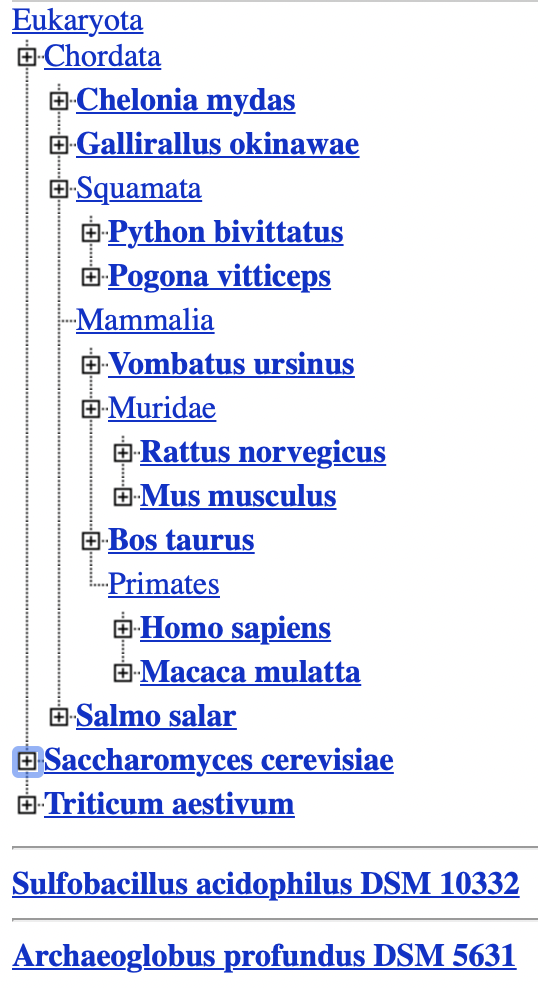
\includegraphics[width=7cm]{images/image9.png}\\
Можно заметить, что это строение очень похоже на деревья, построенные методом наибольшего правдоподобия и методом NJ при выравнивании последовательности алгоритмом Muscle. Поэтому можно сделать вывод, что вышеперечисленные деревья, построенные по одному гену, совпадают с принятыми деревьями видов, а остальные в той или иной мере отличаются.
\end{document}